\documentclass[a4paper]{article}

\usepackage{polski}
\usepackage[utf8]{inputenc}
\usepackage{graphicx}
\usepackage[hidelinks]{hyperref}
\usepackage{listings}
\usepackage{multirow}
\usepackage{color}
\usepackage[labelformat=empty]{caption}

\pagenumbering{arabic}

\title{ITHPC 2014 - raport}
\author{Kacper Siora}
\date{\today}

\begin{document}
\maketitle

\section{Opis zadania}
W ramach laboratorium z przedmiotu \textit{Introduction to High Performance Computing} zrealizowane zostało zadanie 3-cie, czyli mnożenie macierzy przez macierz. Zostały przygotowane trzy wersje programu: sekwencyjna, OpenMP oraz OpenMP dla Xeon Phi. Wszystkie programy i skrypty użyte do rozwiązania zadania można znaleźć w repozytorium \url{https://github.com/Siorski/usa}.

\section{Rozwiązanie}
Stworzone rozwiązania oraz zastosowane w nich kluczowe funkcje:
\begin{itemize}
\item program generujący macierze, wypełniający je losowo liczbami z zakresu od 0 do 100 oraz zapisujący macierze do pliku
\item program mnożący macierze, które zapisane w plikach podawane są jako parametry uruchumieniowe
\item skrypt automatyzujący uruchamianie kolejnych mnożeń
\item dynamiczna alokacja pamięci dla macierzy
\item mierzenie czasu wykonania całego programu, oraz jego kluczowych punktów, tj.  
  \begin{itemize}
  \item wczytywanie danych
  \item główne obliczenia
  \item zapis wyniku
  \end{itemize}
\end{itemize}

\subsection{Mierzenie czasu}
Do mierzenia czasu została użyta biblioteka \textit{time.h} oraz zawarta w niej funkcja \textit{clock\_gettime(CLOCK\_MONOTONIC)}.

\newpage
\subsection{Wersje równoległe}
Stworzenie równoległej wersji rozwiązania sprowadziło się do zrównoleglenia głównej części, w której macierze są mnożone: 
\begin{lstlisting}[language=C,frame=lines,keywordstyle=\color{red}\bfseries
]
#pragma omp parallel shared(macierzA, macierzB, macierzC) private(i,j,k)
  {
    #pragma omp for schedule (static)
    for(i=0; i<ilosc_wierszy_A; i++){
      for(j=0; j<ilosc_kolumn_B; j++){
        for(k=0; k<ilosc_wierszy_B; k++){
          macierzC[i][j] += macierzA[i][k] * macierzB[k][j];
        }
      }
    }
  }
\end{lstlisting}
Wszelkie próby zrównoleglenia fragmentu programu, w którym macierze są wczytywane z, bądź zapisywane do plików przynosiły niestety efekt odwrotny do pożądanego. Program OpenMP uruchamiany był na sigmie, gdzie korzystał on z  8 wątków.

\subsection{Dane testowe}
Do testów działania programu zotało wygenerowanych 6 par macierzy o rozmiarach: 
\begin{description}
  \item[Para 1] 5    x  5    * 5    x  5
  \item[Para 2] 517  x  740  * 740  x  493
  \item[Para 3] 1029 x  1475 * 1475 x  981
  \item[Para 4] 1541 x  2210 * 2210 x  1469
  \item[Para 5] 2053 x  2945 * 2945 x  1957
  \item[Para 6] 2565 x  3680 * 3680 x  2447
\end{description}

\section{Porównanie czasów}
\subsection{Tabele}
Wszystkie czasy w tabelach podane są w sekundach.

\begin{table}[ht!]
\begin{tabular}{l|l|l|l|}
\cline{2-4}
                                                            & \multicolumn{3}{|c|}{\textbf{5x5 * 5x5}}                   \\ \cline{2-4} 
                                                            & \textit{Sekwencyjny} & \textit{OpenMP} & \textit{XEON PHI} \\ \hline
\multicolumn{1}{|l|}{\textit{Czas wczytywania danych}}      & 0,001477             & 0,001588        & 0,000627          \\ \hline
\multicolumn{1}{|l|}{\textit{Czas obliczeń}}                & 0,000002             & 0,000229        & 0,255085          \\ \hline
\multicolumn{1}{|l|}{\textit{Czas zapisu danych}}           & 0,001506             & 0,00099         & 0,000653          \\ \hline
\multicolumn{1}{|l|}{\textit{Czas trwania całego programu}} & 0,003097             & 0,002898        & 0,256662          \\ \hline
\end{tabular}
\end{table}

\begin{table}
\begin{tabular}{l|l|l|l|}
\cline{2-4}
                                                            & \multicolumn{3}{|c|}{\textbf{517x740 * 740x493}}           \\ \cline{2-4} 
                                                            & \textit{Sekwencyjny} & \textit{OpenMP} & \textit{XEON PHI} \\ \hline
\multicolumn{1}{|l|}{\textit{Czas wczytywania danych}}      & 0,085524             & 0,090966        & 0,875284          \\ \hline
\multicolumn{1}{|l|}{\textit{Czas obliczeń}}                & 1,913065             & 0,357867        & 0,26042           \\ \hline
\multicolumn{1}{|l|}{\textit{Czas zapisu danych}}           & 0,074895             & 0,079641        & 0,426752          \\ \hline
\multicolumn{1}{|l|}{\textit{Czas trwania całego programu}} & 2,074703             & 0,529671        & 1,565948          \\ \hline
\end{tabular}
\end{table}

\begin{table}
\begin{tabular}{l|l|l|l|}
\cline{2-4}
                                                            & \multicolumn{3}{|c|}{\textbf{1029x1475 * 1475x981}}        \\ \cline{2-4} 
                                                            & \textit{Sekwencyjny} & \textit{OpenMP} & \textit{XEON PHI} \\ \hline
\multicolumn{1}{|l|}{\textit{Czas wczytywania danych}}      & 0,332428             & 0,336021        & 3,481636          \\ \hline
\multicolumn{1}{|l|}{\textit{Czas obliczeń}}                & 18,193035            & 3,220273        & 0,292785          \\ \hline
\multicolumn{1}{|l|}{\textit{Czas zapisu danych}}           & 0,307626             & 0,322421        & 1,273766          \\ \hline
\multicolumn{1}{|l|}{\textit{Czas trwania całego programu}} & 18,838361            & 3,884008        & 5,060543          \\ \hline
\end{tabular}
\end{table}

\begin{table}
\begin{tabular}{l|l|l|l|}
\cline{2-4}
                                                            & \multicolumn{3}{|c|}{\textbf{1541x2210 * 2210x1469}}       \\ \cline{2-4} 
                                                            & \textit{Sekwencyjny} & \textit{OpenMP} & \textit{XEON PHI} \\ \hline
\multicolumn{1}{|l|}{\textit{Czas wczytywania danych}}      & 0,750734             & 0,752672        & 7,78231           \\ \hline
\multicolumn{1}{|l|}{\textit{Czas obliczeń}}                & 64,640528            & 10,916685       & 0,384762          \\ \hline
\multicolumn{1}{|l|}{\textit{Czas zapisu danych}}           & 0,649202             & 0,687393        & 2,69992           \\ \hline
\multicolumn{1}{|l|}{\textit{Czas trwania całego programu}} & 66,053089            & 12,368927       & 10,892418         \\ \hline
\end{tabular}
\end{table}

\begin{table}
\begin{tabular}{l|l|l|l|}
\cline{2-4}
                                                            & \multicolumn{3}{|c|}{\textbf{2053x2945 * 2945x1957}}       \\ \cline{2-4} 
                                                            & \textit{Sekwencyjny} & \textit{OpenMP} & \textit{XEON PHI} \\ \hline
\multicolumn{1}{|l|}{\textit{Czas wczytywania danych}}      & 1,365159             & 1,308095        & 13,808813         \\ \hline
\multicolumn{1}{|l|}{\textit{Czas obliczeń}}                & 175,745871           & 29,156601       & 0,583053          \\ \hline
\multicolumn{1}{|l|}{\textit{Czas zapisu danych}}           & 1,155145             & 1,204566        & 4,947509          \\ \hline
\multicolumn{1}{|l|}{\textit{Czas trwania całego programu}} & 178,28793            & 31,691602       & 19,382112         \\ \hline
\end{tabular}
\end{table}

\begin{table}
\begin{tabular}{l|l|l|l|}
\cline{2-4}
                                                            & \multicolumn{3}{|c|}{\textbf{2565x3680 * 3680x2447}}       \\ \cline{2-4} 
                                                            & \textit{Sekwencyjny} & \textit{OpenMP} & \textit{XEON PHI} \\ \hline
\multicolumn{1}{|l|}{\textit{Czas wczytywania danych}}      & 2,042326             & 2,037463        & 21,647846         \\ \hline
\multicolumn{1}{|l|}{\textit{Czas obliczeń}}                & 346,049103            & 59,394568       & 0,922356          \\ \hline
\multicolumn{1}{|l|}{\textit{Czas zapisu danych}}           & 1,741209             & 1,863713        & 7,723572          \\ \hline
\multicolumn{1}{|l|}{\textit{Czas trwania całego programu}} & 349,253795           & 60,331661       & 30,358427         \\ \hline
\end{tabular}
\end{table}

\subsection{Wykresy}
\begin{figure}[h!]
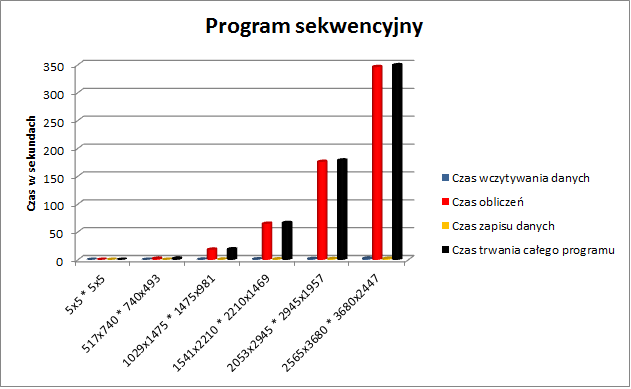
\includegraphics[width=1\textwidth]{sekw.png}
\caption{Wykres z czasami wykonania programu sekwencyjnego.}
\end{figure}

\begin{figure}[h!]
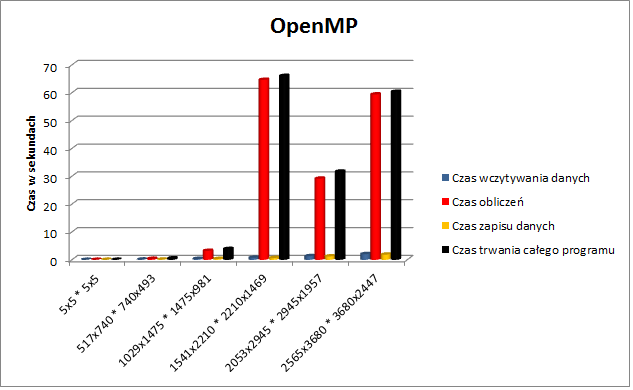
\includegraphics[width=1\textwidth]{OpenMP.png}
\caption{Wykres z czasami wykonania programu OpenMP.}
\end{figure}

\begin{figure}
\includegraphics[width=1\textwidth]{Xeon_Phi.png}
\caption{Wykres z czasami wykonania programu na Xeon Phi.}
\end{figure}

\newpage
\section {Wnioski}
Z wykresów oraz tabel, można jednoznaczenie odczytać, iż programy wykonywane na Xeonie Phi działają najszybciej, co nie jest oczywiście żadnym zaskoczeniem. Dla małych macierzy różnice są jeszcze niezbyt znaczące, natomiast już dla największych macierzy jakie zostały przetestowane przyspieszenie jest widoczne - 2-krotnie szybciej niż program OpenMP oraz ponad 11-krotnie szybciej niż program sekwencyjny. Dwóm pierwszym programom najwięcej czasu zajmują główne obliczenia (ponad 90 \% czasu). Xeon Phi natomiast na same obliczenia poświęca najmniej uwagi - zaledwie 3\%. Zdecydowanie bardziej zajmujące dla procesora Intel jest wczytywanie danych oraz w mniejszym, ale nadal znacznym stopniu ich zapisywanie. Zatem sytuacja ma się zupełnie odwrotnie w przypadku programu sekwencyjnego oraz OpenMP w porównaniu do programu uruchamianego na procesorze Xeon Phi.
\end{document}